%- - - - - - - - - - - - - - - - - - - - - - - - - - - - - - - - - 
\subsection{Data Acquisition}

\textbf{\emph{Jan B.}}

\emph{This section does not need to go into complete detail on the DAQ system (that should be in a different document). This should include the global picture (see slide 5 of Jin's intro talk at AI4EIC or slide 3 of Fernando's talk). What is needed here is the expected overall data rate and how many streams. The current plan is to implement a first stage HLT which may or may not require full event building. This section will need to include an estimate of how much reduction the first stage HLT will provide (i.e. what is the data rate going into the calibration system.}

\emph{Also, do we implement the first stage HLT in FPGAs or on CPU/GPU? Need estimates on how much compute resource will be needed for first stage HLT.}

%--------------------------------------------------------------------
Figure \ref{fig:data_acquisition_diagram} illustrates a concept of the data acquisition system with some estimated rates.

\begin{figure}[hbt!]
 \begin{center}
   \raisebox{0.5mm}{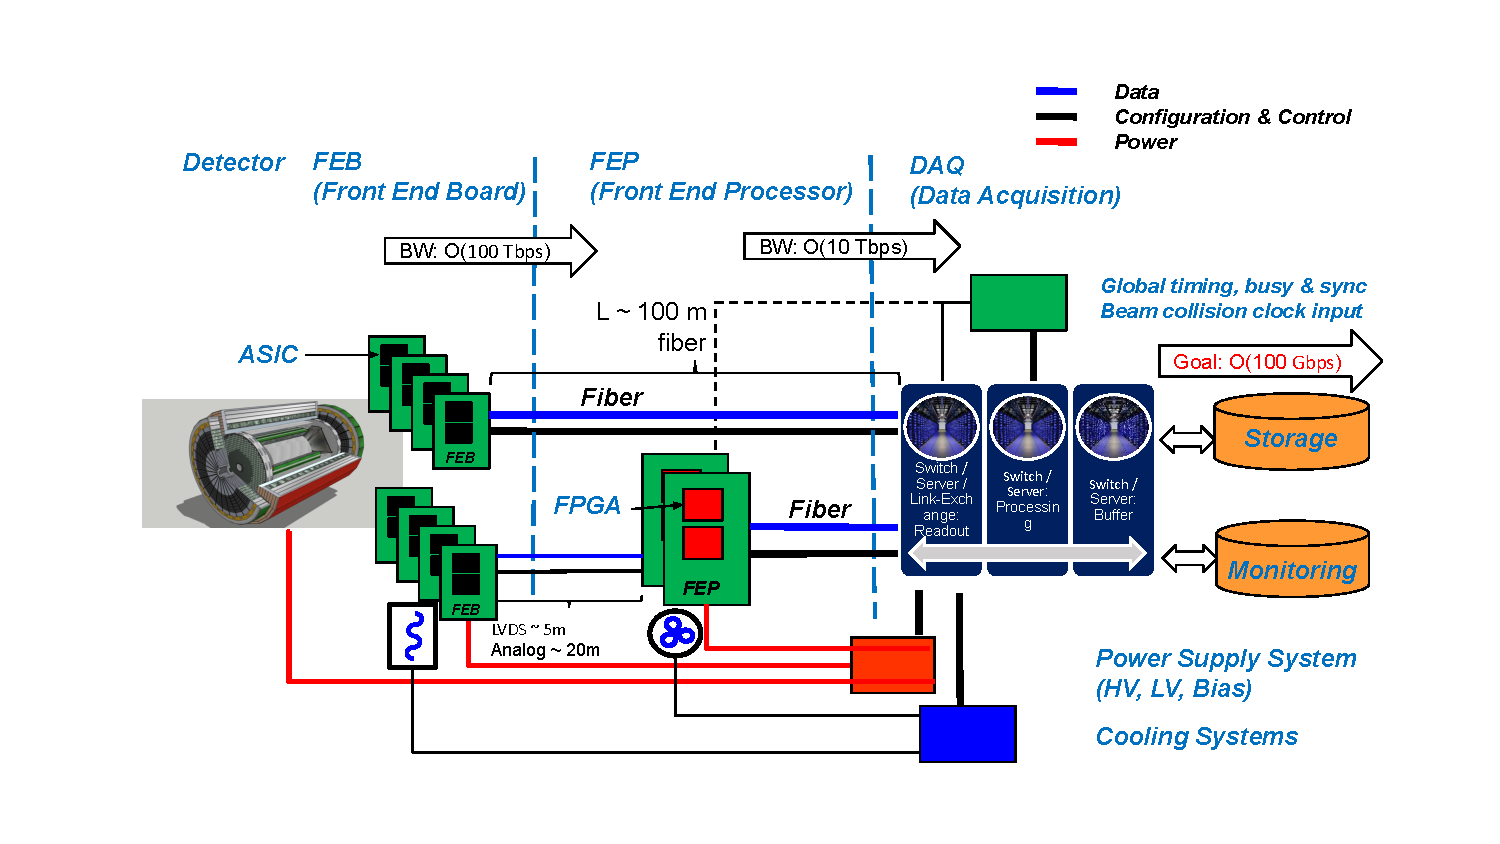
\includegraphics[trim=50 30 50 30, clip, width=0.99\linewidth]{figs/figure_data_acquisition_diagram.pdf}}
  \caption[Data Acquisition Diagram]{\label{fig:data_acquisition_diagram} Diagram of a Data Acquisition system. This is reproduced from slides shown at AI4EIC 2021\cite{EIC_readout_overview_AI4EIC_2021}. }
 \end{center}
\end{figure}

%- - - - - - - - - - - - - - - - - - - - - - - - - - - - - - - - - 
\subsection{Monitoring}

Hydra\cite{Hydra2021}
